\documentclass[12pt]{article}
\usepackage[utf8]{inputenc}
\usepackage{float}
\usepackage{amsmath}


\usepackage[hmargin=3cm,vmargin=6.0cm]{geometry}
%\topmargin=0cm
\topmargin=-2cm
\addtolength{\textheight}{6.5cm}
\addtolength{\textwidth}{2.0cm}
%\setlength{\leftmargin}{-5cm}
\setlength{\oddsidemargin}{0.0cm}
\setlength{\evensidemargin}{0.0cm}

%misc libraries goes here
\usepackage{tikz}
\usetikzlibrary{automata,positioning}

\begin{document}

\section*{Student Information } 
%Write your full name and id number between the colon and newline
%Put one empty space character after colon and before newline
Full Name :  Adil Kaan akan \\
Id Number :  2171155 \\

% Write your answers below the section tags
\section*{Answer 1}

\subsection*{a.}
We can prove with a method that is as follows. \\
The method uses an integer as a denominator and gives all integers that is less than that denominator as numerator. For the listing, the method uses reverse diagonals such that -1/2,-1/3,-2/3,-1/4,-1/5,-2/4,..\\ \\ \\ \\
-1/2 \\
-1/3 -2/3 \\
-1/4 -2/4 -3/4 \\
-1/5 -2/5 -3/5 -4/5 \\
...


We can write infinitely many rows if we increment the denominator one by one. Since there are infinitely many rows, there are infinitely many rational number in interval (-1,0). Since the method allows us to list the number by using the diagonals, we can list them to have one to one correspondence between natural numbers. Therefore, we can say that the rational numbers in the open interval which is (-1,0) have the same cardinality with natural numbers and are countably infinite.



\subsection*{b.}
If the given language L is a regular language, then it must be accepted by the finite automaton. We can build a finite automata to accept the $L^+$. Since the $L^+$ is $L \circ L^*$, we can use the kleene star and concentanation. Since all finite languages are regular,we can build a finite automata that has finite states to accept finite language, we can say that L is regular. Since the kleene star operation and concatenation operation are closures, we can say that if we L is regular then $L^*$ is regular and $L \circ L$ is also regular. By using that, we can say that $L \circ L^*$ is a regular language. Since the $L^+$ is $L\circ L^*$, the all of the finite languages, say L, all the $L^+$ are regular. Therefore, the set $D = \{ L^+ :$ finite regular language over the unary alphabet $\sum = \{ a \}$ and $L^+$ is not regular is emptyset.

\subsection*{c.}
The set of all languages contains the regular languages and the languages that are not regulaer, actually it is union of them. It is uncountable since there are countably infinite alphabet and the cardinality of all languages is $2^{|\sum^*|}$ and that means uncountability. Since the regular languages are countably infinite and the set of all languages is uncountable, the set of non regular languages must be uncountable to the set of all languages be uncountable. Then, we can say that the set of languages that are not regular is uncountable.



\section*{Answer 2}
\subsection*{a.}


\begin{center}
\begin{tikzpicture}[scale=0.2]
\tikzstyle{every node}+=[inner sep=0pt]
\draw [black] (15.8,-7.8) circle (3);
\draw (15.8,-7.8) node {$q_0$};
\draw [black] (45.2,-11.6) circle (3);
\draw (45.2,-11.6) node {$q_1$};
\draw [black] (45.2,-11.6) circle (2.4);
\draw [black] (17,-32.5) circle (3);
\draw (17,-32.5) node {$q_2$};
\draw [black] (17,-32.5) circle (2.4);
\draw [black] (59.4,-30.5) circle (3);
\draw (59.4,-30.5) node {$q_3$};
\draw [black] (59.4,-30.5) circle (2.4);
\draw [black] (46.2,-50.8) circle (3);
\draw (46.2,-50.8) node {$q_4$};
\draw [black] (8.5,-7.8) -- (12.8,-7.8);
\draw (8,-7.8) node [left] {$start$};
\fill [black] (12.8,-7.8) -- (12,-7.3) -- (12,-8.3);
\draw [black] (18.78,-8.18) -- (42.22,-11.22);
\fill [black] (42.22,-11.22) -- (41.5,-10.62) -- (41.37,-11.61);
\draw (30.22,-10.29) node [below] {$a$};
\draw [black] (15.95,-10.8) -- (16.85,-29.5);
\fill [black] (16.85,-29.5) -- (17.32,-28.68) -- (16.32,-28.73);
\draw (15.83,-20.17) node [left] {$b$};
\draw [black] (44.967,-8.621) arc (212.19859:-75.80141:2.25);
\draw (48.61,-4.82) node [above] {$a$};
\fill [black] (47.42,-9.6) -- (48.37,-9.6) -- (47.83,-8.75);
\draw [black] (14.505,-34.145) arc (-28.87498:-316.87498:2.25);
\draw (9.63,-33.47) node [left] {$b$};
\fill [black] (14.18,-31.52) -- (13.72,-30.7) -- (13.23,-31.57);
\draw [black] (19.54,-34.09) -- (43.66,-49.21);
\fill [black] (43.66,-49.21) -- (43.25,-48.36) -- (42.71,-49.21);
\draw (30.66,-42.15) node [below] {$a$};
\draw [black] (47,-14) -- (57.6,-28.1);
\fill [black] (57.6,-28.1) -- (57.52,-27.16) -- (56.72,-27.76);
\draw (51.72,-22.45) node [left] {$b$};
\draw [black] (58.818,-33.442) arc (-14.17157:-51.89601:28.84);
\fill [black] (48.65,-49.07) -- (49.59,-48.97) -- (48.97,-48.19);
\draw (55.65,-43.42) node [right] {$b$};
\draw [black] (47.109,-47.942) arc (160.21448:133.71794:40.212);
\fill [black] (47.11,-47.94) -- (47.85,-47.36) -- (46.91,-47.02);
\draw (50.62,-38.31) node [left] {$a$};
\draw [black] (49.165,-51.173) arc (110.56723:-177.43277:2.25);
\draw (52.45,-55.85) node [right] {$a$};
\fill [black] (47.71,-53.38) -- (47.52,-54.3) -- (48.46,-53.95);
\draw [black] (45.168,-53.604) arc (7.5312:-280.4688:2.25);
\draw (40.78,-56.92) node [left] {$b$};
\fill [black] (43.35,-51.69) -- (42.49,-51.3) -- (42.62,-52.29);
\end{tikzpicture}
\end{center}


\subsection*{b.}

\begin{center}
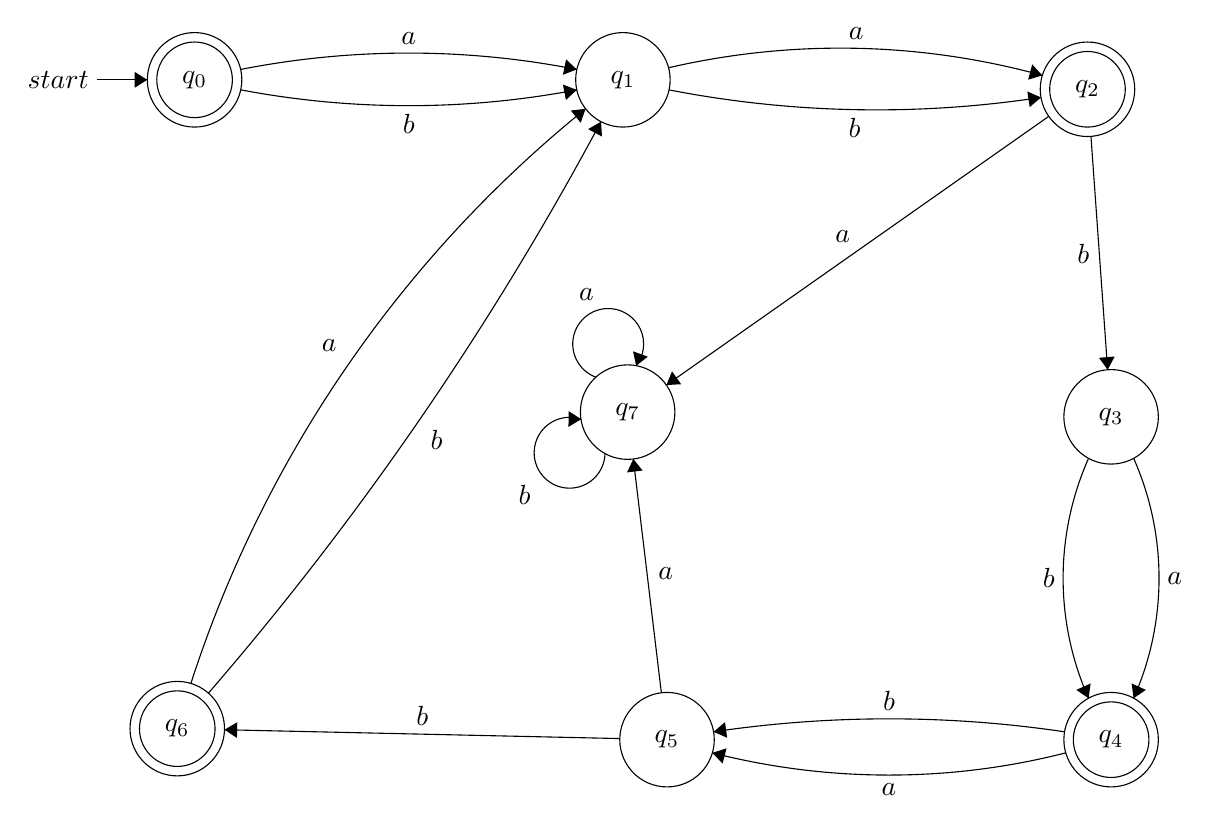
\begin{tikzpicture}[scale=0.2]
\tikzstyle{every node}+=[inner sep=0pt]
\draw [black] (10.7,-8.2) circle (3);
\draw (10.7,-8.2) node {$q_0$};
\draw [black] (10.7,-8.2) circle (2.4);
\draw [black] (37.9,-8.2) circle (3);
\draw (37.9,-8.2) node {$q_1$};
\draw [black] (67.4,-8.8) circle (3);
\draw (67.4,-8.8) node {$q_2$};
\draw [black] (67.4,-8.8) circle (2.4);
\draw [black] (68.9,-29.6) circle (3);
\draw (68.9,-29.6) node {$q_3$};
\draw [black] (68.9,-50.1) circle (3);
\draw (68.9,-50.1) node {$q_4$};
\draw [black] (68.9,-50.1) circle (2.4);
\draw [black] (40.7,-50.1) circle (3);
\draw (40.7,-50.1) node {$q_5$};
\draw [black] (9.6,-49.4) circle (3);
\draw (9.6,-49.4) node {$q_6$};
\draw [black] (9.6,-49.4) circle (2.4);
\draw [black] (38.2,-29.3) circle (3);
\draw (38.2,-29.3) node {$q_7$};
\draw [black] (13.626,-7.541) arc (101.13954:78.86046:55.247);
\fill [black] (34.97,-7.54) -- (34.29,-6.9) -- (34.09,-7.88);
\draw (24.3,-6) node [above] {$a$};
\draw [black] (34.969,-8.837) arc (-79.23699:-100.76301:57.13);
\fill [black] (34.97,-8.84) -- (34.09,-8.5) -- (34.28,-9.48);
\draw (24.3,-10.34) node [below] {$b$};
\draw [black] (4.5,-8.2) -- (7.7,-8.2);
\draw (4,-8.2) node [left] {$start$};
\fill [black] (7.7,-8.2) -- (6.9,-7.7) -- (6.9,-8.7);
\draw [black] (40.8,-7.433) arc (103.04119:74.62845:48.365);
\fill [black] (64.53,-7.92) -- (63.89,-7.22) -- (63.63,-8.19);
\draw (52.71,-5.68) node [above] {$a$};
\draw [black] (64.445,-9.317) arc (-81.32704:-101.00332:69.114);
\fill [black] (64.45,-9.32) -- (63.58,-8.94) -- (63.73,-9.93);
\draw (52.61,-10.61) node [below] {$b$};
\draw [black] (67.62,-11.79) -- (68.68,-26.61);
\fill [black] (68.68,-26.61) -- (69.13,-25.77) -- (68.13,-25.85);
\draw (67.55,-19.25) node [left] {$b$};
\draw [black] (64.94,-10.52) -- (40.66,-27.58);
\fill [black] (40.66,-27.58) -- (41.6,-27.53) -- (41.02,-26.71);
\draw (51.85,-18.55) node [above] {$a$};
\draw [black] (70.33,-32.234) arc (23.91968:-23.91968:18.784);
\fill [black] (70.33,-47.47) -- (71.11,-46.94) -- (70.2,-46.53);
\draw (72.44,-39.85) node [right] {$a$};
\draw [black] (67.468,-47.468) arc (-156.03562:-203.96438:18.755);
\fill [black] (67.47,-47.47) -- (67.6,-46.53) -- (66.69,-46.94);
\draw (65.35,-39.85) node [left] {$b$};
\draw [black] (66.02,-50.938) arc (-75.66941:-104.33059:45.33);
\fill [black] (43.58,-50.94) -- (44.23,-51.62) -- (44.48,-50.65);
\draw (54.8,-52.85) node [below] {$a$};
\draw [black] (43.658,-49.6) arc (98.4583:81.5417:75.751);
\fill [black] (43.66,-49.6) -- (44.52,-49.98) -- (44.38,-48.99);
\draw (54.8,-48.28) node [above] {$b$};
\draw [black] (40.34,-47.12) -- (38.56,-32.28);
\fill [black] (38.56,-32.28) -- (38.16,-33.13) -- (39.15,-33.01);
\draw (40.12,-39.58) node [right] {$a$};
\draw [black] (37.7,-50.03) -- (12.6,-49.47);
\fill [black] (12.6,-49.47) -- (13.39,-49.99) -- (13.41,-48.99);
\draw (25.16,-49.23) node [above] {$b$};
\draw [black] (10.466,-46.528) arc (162.10871:128.92147:77.505);
\fill [black] (35.53,-10.04) -- (34.59,-10.15) -- (35.22,-10.93);
\draw (19.74,-25.1) node [left] {$a$};
\draw [black] (36.506,-10.856) arc (-28.12795:-40.84187:198.81);
\fill [black] (36.51,-10.86) -- (35.69,-11.33) -- (36.57,-11.8);
\draw (25.65,-31.05) node [right] {$b$};
\draw [black] (36.192,-27.087) arc (249.9454:-38.0546:2.25);
\draw (35.58,-22.26) node [above] {$a$};
\fill [black] (38.74,-26.36) -- (39.48,-25.78) -- (38.54,-25.44);
\draw [black] (36.762,-31.92) arc (-1.02185:-289.02185:2.25);
\draw (32.07,-34.53) node [left] {$b$};
\fill [black] (35.25,-29.75) -- (34.46,-29.24) -- (34.44,-30.24);
\end{tikzpicture}
\end{center}


\subsection*{c.}

\begin{center}
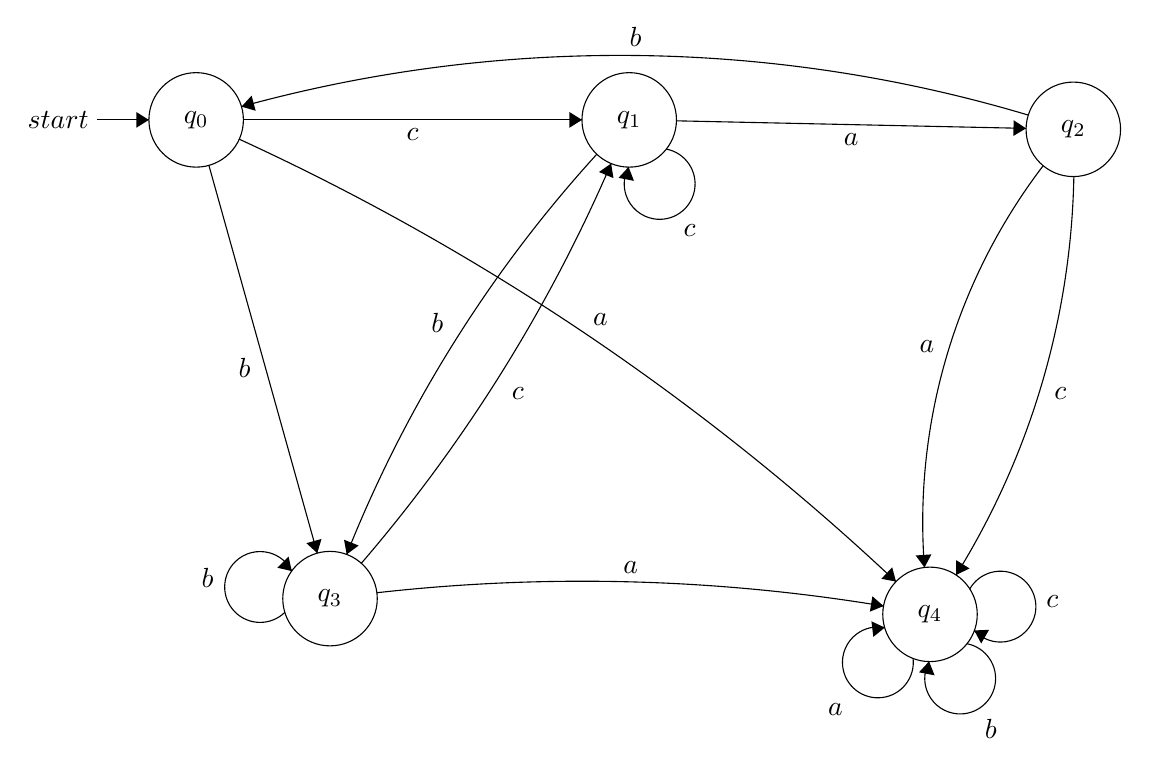
\begin{tikzpicture}[scale=0.2]
\tikzstyle{every node}+=[inner sep=0pt]
\draw [black] (11.6,-8.2) circle (3);
\draw (11.6,-8.2) node {$q_0$};
\draw [black] (39.1,-8.2) circle (3);
\draw (39.1,-8.2) node {$q_1$};
\draw [black] (67.3,-8.8) circle (3);
\draw (67.3,-8.8) node {$q_2$};
\draw [black] (20.1,-38.6) circle (3);
\draw (20.1,-38.6) node {$q_3$};
\draw [black] (58.2,-39.6) circle (3);
\draw (58.2,-39.6) node {$q_4$};
\draw [black] (5.3,-8.2) -- (8.6,-8.2);
\draw (4.8,-8.2) node [left] {$start$};
\fill [black] (8.6,-8.2) -- (7.8,-7.7) -- (7.8,-8.7);
\draw [black] (14.6,-8.2) -- (36.1,-8.2);
\fill [black] (36.1,-8.2) -- (35.3,-7.7) -- (35.3,-8.7);
\draw (25.35,-8.7) node [below] {$c$};
\draw [black] (12.41,-11.09) -- (19.29,-35.71);
\fill [black] (19.29,-35.71) -- (19.56,-34.81) -- (18.6,-35.08);
\draw (15.08,-23.95) node [left] {$b$};
\draw [black] (14.338,-9.426) arc (65.33165:46.72261:155.492);
\fill [black] (56.04,-37.52) -- (55.8,-36.61) -- (55.11,-37.34);
\draw (37.28,-21.28) node [above] {$a$};
\draw [black] (41.445,-10.053) arc (79.41733:-208.58267:2.25);
\draw (42.93,-14.8) node [below] {$c$};
\fill [black] (39.06,-11.19) -- (38.42,-11.88) -- (39.4,-12.07);
\draw [black] (42.1,-8.26) -- (64.3,-8.74);
\fill [black] (64.3,-8.74) -- (63.51,-8.22) -- (63.49,-9.22);
\draw (53.19,-9.02) node [below] {$a$};
\draw [black] (21.158,-35.793) arc (158.31316:137.67607:83.649);
\fill [black] (21.16,-35.79) -- (21.92,-35.23) -- (20.99,-34.86);
\draw (27.32,-21.08) node [left] {$b$};
\draw [black] (14.478,-7.355) arc (105.40439:73.36128:90.516);
\fill [black] (14.48,-7.36) -- (15.38,-7.62) -- (15.12,-6.66);
\draw (39.5,-3.6) node [above] {$b$};
\draw [black] (57.848,-36.621) arc (-175.5728:-217.34723:37.308);
\fill [black] (57.85,-36.62) -- (58.29,-35.79) -- (57.29,-35.86);
\draw (58.5,-22.58) node [left] {$a$};
\draw [black] (67.334,-11.799) arc (-1.08567:-31.83436:49.755);
\fill [black] (59.86,-37.1) -- (60.71,-36.68) -- (59.86,-36.16);
\draw (66.07,-25.55) node [right] {$c$};
\draw [black] (57.124,-42.388) arc (6.631:-281.369:2.25);
\draw (52.7,-45.63) node [left] {$a$};
\fill [black] (55.33,-40.44) -- (54.48,-40.04) -- (54.6,-41.03);
\draw [black] (60.537,-41.462) arc (79.19646:-208.80354:2.25);
\draw (62.06,-46.21) node [below] {$b$};
\fill [black] (58.14,-42.59) -- (57.5,-43.28) -- (58.49,-43.47);
\draw [black] (60.719,-37.993) arc (150.26702:-137.73298:2.25);
\draw (65.56,-38.76) node [right] {$c$};
\fill [black] (61.01,-40.62) -- (61.45,-41.45) -- (61.95,-40.58);
\draw [black] (17.239,-39.464) arc (314.53768:26.53768:2.25);
\draw (12.73,-37.26) node [left] {$b$};
\fill [black] (17.67,-36.85) -- (17.47,-35.93) -- (16.76,-36.64);
\draw [black] (37.954,-10.972) arc (-23.32979:-40.68098:99.219);
\fill [black] (37.95,-10.97) -- (37.18,-11.51) -- (38.1,-11.9);
\draw (31.61,-25.56) node [right] {$c$};
\draw [black] (23.077,-38.226) arc (96.42103:80.57201:116.712);
\fill [black] (55.25,-39.07) -- (54.54,-38.45) -- (54.38,-39.43);
\draw (39.2,-37.01) node [above] {$a$};
\end{tikzpicture}
\end{center}







\section*{Answer 3}


\subsection*{a.}
$(q_0,abbb) \vdash_N (q_1,bbb) \vdash_N (q_2,bb)$ \\
$(q_0,abbb) \vdash_N (q_2,abbb) \vdash_N (q_4,bbb) \vdash_N (q_3,bb) \vdash_N (q_3,b),(q_4,e)$ \\
$(q_0,abbb)\vdash_N (q_1,bbb) \vdash_N (q_3,bb) \vdash_N (q_3,b) \vdash_N (q_3,e) $ \\

On the above, there are some of the ways which experessing the string "abbb" and all of them end on the $q_3$ or $q_4$ state.
Since only accepting state is $q_5$ and there is no way to reach from $q_3$ and$q_4 $ to $q_5$, there is no way to accept "abbb" string.


\subsection*{b.}
$(q_0,ababa) \vdash_N (q_1,baba) \vdash_N (q_2,aba) \vdash_N (q_4, ba) \vdash_N (q_3, a) \vdash_N (q_5, e)$ and also
$(q_0,ababa) \vdash_N (q_2, ababa) \vdash_N (q_4,baba) \vdash_N (q_3,aba) \vdash_N (q_1 ba) \vdash_N (q_3, ba) \vdash_N (q_3, a) \vdash_N (q_5,e)$
Since both of the configurations end in the $q_5$ which accept state of the N, the string "ababa" accepted by the N.




\section*{Answer 4}

\subsection*{a.}

We should add a new start state which is $q_4$ and a new final state which is $q_5$ in order to do state elimination. Moreover, we should add empty transitions from new start states, $q_4$, and to new final state ,$q_5$. After doing these operations the corresponding NFA is as follows:

\begin{center}
\begin{tikzpicture}[scale=0.2]
\tikzstyle{every node}+=[inner sep=0pt]
\draw [black] (11.8,-8.2) circle (3);
\draw (11.8,-8.2) node {$q_4$};
\draw [black] (37.2,-8.7) circle (3);
\draw (37.2,-8.7) node {$q_0$};
\draw [black] (24.3,-29.3) circle (3);
\draw (24.3,-29.3) node {$q_2$};
\draw [black] (66.5,-17.9) circle (3);
\draw (66.5,-17.9) node {$q_1$};
\draw [black] (41.8,-49.6) circle (3);
\draw (41.8,-49.6) node {$q_5$};
\draw [black] (41.8,-49.6) circle (2.4);
\draw [black] (67.7,-43.2) circle (3);
\draw (67.7,-43.2) node {$q_3$};
\draw [black] (5.5,-8.2) -- (8.8,-8.2);
\draw (5,-8.2) node [left] {$start$};
\fill [black] (8.8,-8.2) -- (8,-7.7) -- (8,-8.7);
\draw [black] (14.8,-8.26) -- (34.2,-8.64);
\fill [black] (34.2,-8.64) -- (33.41,-8.13) -- (33.39,-9.13);
\draw (24.49,-8.97) node [below] {$e$};
\draw [black] (40.06,-9.6) -- (63.64,-17);
\fill [black] (63.64,-17) -- (63.02,-16.28) -- (62.72,-17.24);
\draw (50.99,-13.84) node [below] {$b$};
\draw [black] (25.89,-26.76) -- (35.61,-11.24);
\fill [black] (35.61,-11.24) -- (34.76,-11.66) -- (35.61,-12.19);
\draw (31.38,-20.29) node [right] {$a$};
\draw [black] (26.871,-27.754) arc (119.86814:90.36619:74.509);
\fill [black] (26.87,-27.75) -- (27.81,-27.79) -- (27.32,-26.92);
\draw (43.82,-19.88) node [above] {$a$};
\draw [black] (63.79,-19.186) arc (-65.36894:-84.39673:114.374);
\fill [black] (63.79,-19.19) -- (62.85,-19.06) -- (63.27,-19.97);
\draw (46.72,-26.2) node [below] {$b$};
\draw [black] (65.816,-40.869) arc (-145.46448:-209.10442:19.435);
\fill [black] (65.82,-40.87) -- (65.77,-39.93) -- (64.95,-40.49);
\draw (61.84,-30.79) node [left] {$e$};
\draw [black] (68.102,-20.434) arc (28.57895:-23.14785:23.055);
\fill [black] (68.1,-20.43) -- (68.05,-21.38) -- (68.92,-20.9);
\draw (71.46,-30.35) node [right] {$b$};
\draw [black] (70.38,-41.877) arc (144:-144:2.25);
\draw (74.95,-43.2) node [right] {$a$};
\fill [black] (70.38,-44.52) -- (70.73,-45.4) -- (71.32,-44.59);
\draw [black] (26.26,-31.57) -- (39.84,-47.33);
\fill [black] (39.84,-47.33) -- (39.7,-46.4) -- (38.94,-47.05);
\draw (32.5,-40.9) node [left] {$e$};
\draw [black] (21.422,-30.106) arc (313.38034:25.38034:2.25);
\draw (16.94,-27.78) node [left] {$b$};
\fill [black] (21.91,-27.51) -- (21.72,-26.58) -- (21,-27.27);
\draw [black] (64.79,-43.92) -- (44.71,-48.88);
\fill [black] (44.71,-48.88) -- (45.61,-49.17) -- (45.37,-48.2);
\draw (54.08,-45.83) node [above] {$e$};
\draw [black] (27.16,-30.22) -- (64.84,-42.28);
\fill [black] (64.84,-42.28) -- (64.23,-41.56) -- (63.93,-42.52);
\draw (45.13,-36.79) node [below] {$b$};
\end{tikzpicture}
\end{center}

\subsection*{b.}

Now i will eliminate states one by one and draw the GFA corresponding to the eliminated state.

After eliminating $q_0$ state, we get GFA which follows.

\begin{center}
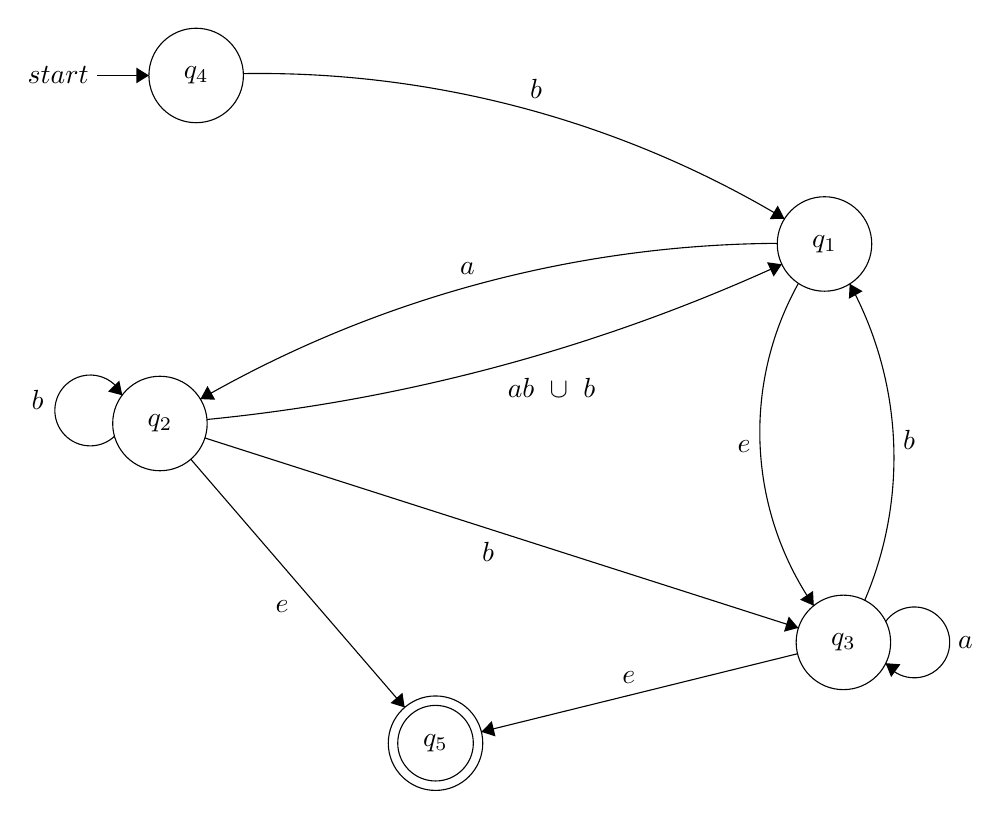
\begin{tikzpicture}[scale=0.2]
\tikzstyle{every node}+=[inner sep=0pt]
\draw [black] (26.6,-7.2) circle (3);
\draw (26.6,-7.2) node {$q_4$};
\draw [black] (24.3,-29.3) circle (3);
\draw (24.3,-29.3) node {$q_2$};
\draw [black] (66.5,-17.9) circle (3);
\draw (66.5,-17.9) node {$q_1$};
\draw [black] (41.8,-49.6) circle (3);
\draw (41.8,-49.6) node {$q_5$};
\draw [black] (41.8,-49.6) circle (2.4);
\draw [black] (67.7,-43.2) circle (3);
\draw (67.7,-43.2) node {$q_3$};
\draw [black] (20.3,-7.2) -- (23.6,-7.2);
\draw (19.8,-7.2) node [left] {$start$};
\fill [black] (23.6,-7.2) -- (22.8,-6.7) -- (22.8,-7.7);
\draw [black] (26.871,-27.754) arc (119.86814:90.36619:74.509);
\fill [black] (26.87,-27.75) -- (27.81,-27.79) -- (27.32,-26.92);
\draw (43.82,-19.88) node [above] {$a$};
\draw [black] (63.79,-19.186) arc (-65.36894:-84.39673:114.374);
\fill [black] (63.79,-19.19) -- (62.85,-19.06) -- (63.27,-19.97);
\draw (49.17,-26.39) node [below] {$ab\mbox{ }\cup\mbox{ }b$};
\draw [black] (65.816,-40.869) arc (-145.46448:-209.10442:19.435);
\fill [black] (65.82,-40.87) -- (65.77,-39.93) -- (64.95,-40.49);
\draw (61.84,-30.79) node [left] {$e$};
\draw [black] (68.102,-20.434) arc (28.57895:-23.14785:23.055);
\fill [black] (68.1,-20.43) -- (68.05,-21.38) -- (68.92,-20.9);
\draw (71.46,-30.35) node [right] {$b$};
\draw [black] (70.38,-41.877) arc (144:-144:2.25);
\draw (74.95,-43.2) node [right] {$a$};
\fill [black] (70.38,-44.52) -- (70.73,-45.4) -- (71.32,-44.59);
\draw [black] (26.26,-31.57) -- (39.84,-47.33);
\fill [black] (39.84,-47.33) -- (39.7,-46.4) -- (38.94,-47.05);
\draw (32.5,-40.9) node [left] {$e$};
\draw [black] (21.422,-30.106) arc (313.38034:25.38034:2.25);
\draw (16.94,-27.78) node [left] {$b$};
\fill [black] (21.91,-27.51) -- (21.72,-26.58) -- (21,-27.27);
\draw [black] (64.79,-43.92) -- (44.71,-48.88);
\fill [black] (44.71,-48.88) -- (45.61,-49.17) -- (45.37,-48.2);
\draw (54.08,-45.83) node [above] {$e$};
\draw [black] (27.16,-30.22) -- (64.84,-42.28);
\fill [black] (64.84,-42.28) -- (64.23,-41.56) -- (63.93,-42.52);
\draw (45.13,-36.79) node [below] {$b$};
\draw [black] (29.597,-7.082) arc (90.9206:59.05574:64.809);
\fill [black] (63.96,-16.3) -- (63.53,-15.46) -- (63.02,-16.32);
\draw (48.19,-8.72) node [above] {$b$};
\end{tikzpicture}
\end{center}

Then when eliminate the $q_1$ the corresponding GFA as follows

\begin{center}
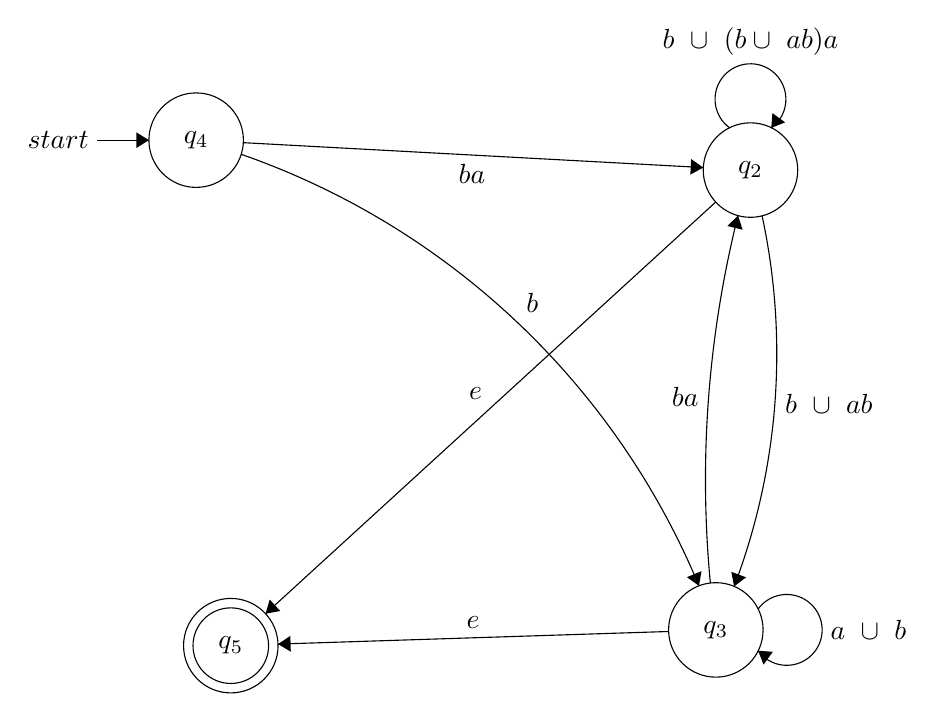
\begin{tikzpicture}[scale=0.2]
\tikzstyle{every node}+=[inner sep=0pt]
\draw [black] (29.8,-12.8) circle (3);
\draw (29.8,-12.8) node {$q_4$};
\draw [black] (65,-14.7) circle (3);
\draw (65,-14.7) node {$q_2$};
\draw [black] (32,-44.9) circle (3);
\draw (32,-44.9) node {$q_5$};
\draw [black] (32,-44.9) circle (2.4);
\draw [black] (62.8,-43.9) circle (3);
\draw (62.8,-43.9) node {$q_3$};
\draw [black] (23.5,-12.8) -- (26.8,-12.8);
\draw (23,-12.8) node [left] {$start$};
\fill [black] (26.8,-12.8) -- (26,-12.3) -- (26,-13.3);
\draw [black] (65.48,-42.577) arc (144:-144:2.25);
\draw (70.05,-43.9) node [right] {$a\mbox{ }\cup\mbox{ }b$};
\fill [black] (65.48,-45.22) -- (65.83,-46.1) -- (66.42,-45.29);
\draw [black] (62.79,-16.73) -- (34.21,-42.87);
\fill [black] (34.21,-42.87) -- (35.14,-42.7) -- (34.47,-41.97);
\draw (47.54,-29.31) node [above] {$e$};
\draw [black] (63.677,-12.02) arc (234:-54:2.25);
\draw (65,-7.45) node [above] {$b\mbox{ }\cup\mbox{ }(b\cup\mbox{ }ab)a$};
\fill [black] (66.32,-12.02) -- (67.2,-11.67) -- (66.39,-11.08);
\draw [black] (59.8,-44) -- (35,-44.8);
\fill [black] (35,-44.8) -- (35.81,-45.28) -- (35.78,-44.28);
\draw (47.38,-43.87) node [above] {$e$};
\draw [black] (65.737,-17.608) arc (12.151:-20.76833:41.637);
\fill [black] (63.96,-41.14) -- (64.72,-40.56) -- (63.78,-40.21);
\draw (67.16,-29.55) node [right] {$b\mbox{ }\cup\mbox{ }ab$};
\draw [black] (32.661,-13.7) arc (70.78188:22.61376:48.945);
\fill [black] (61.73,-41.1) -- (61.89,-40.17) -- (60.96,-40.55);
\draw (51.14,-23.81) node [above] {$b$};
\draw [black] (32.8,-12.96) -- (62,-14.54);
\fill [black] (62,-14.54) -- (61.23,-14) -- (61.18,-14.99);
\draw (47.31,-14.32) node [below] {$ba$};
\draw [black] (62.452,-40.921) arc (-174.57311:-194.04422:69.169);
\fill [black] (64.21,-17.59) -- (63.53,-18.25) -- (64.5,-18.49);
\draw (61.73,-29.13) node [left] {$ba$};
\end{tikzpicture}
\end{center}

After eliminating $q_2$, corresponding GFA as follows

\begin{center}
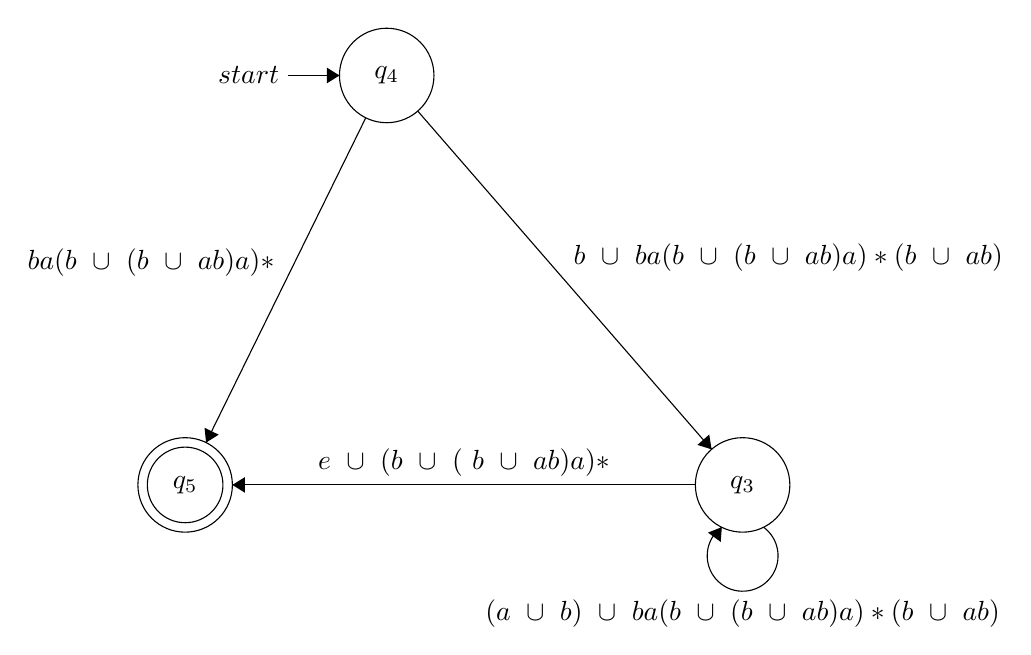
\begin{tikzpicture}[scale=0.2]
\tikzstyle{every node}+=[inner sep=0pt]
\draw [black] (33.4,-11) circle (3);
\draw (33.4,-11) node {$q_4$};
\draw [black] (20.6,-37) circle (3);
\draw (20.6,-37) node {$q_5$};
\draw [black] (20.6,-37) circle (2.4);
\draw [black] (56,-37) circle (3);
\draw (56,-37) node {$q_3$};
\draw [black] (27.1,-11) -- (30.4,-11);
\draw (26.6,-11) node [left] {$start$};
\fill [black] (30.4,-11) -- (29.6,-10.5) -- (29.6,-11.5);
\draw [black] (57.323,-39.68) arc (54:-234:2.25);
\draw (56,-44.25) node [below] {$(a\mbox{ }\cup\mbox{ }b)\mbox{ }\cup\mbox{ }ba(b\mbox{ }\cup\mbox{ }(b\mbox{ }\cup\mbox{ }ab)a)*(b\mbox{ }\cup\mbox{ }ab)$};
\fill [black] (54.68,-39.68) -- (53.8,-40.03) -- (54.61,-40.62);
\draw [black] (53,-37) -- (23.6,-37);
\fill [black] (23.6,-37) -- (24.4,-37.5) -- (24.4,-36.5);
\draw (38.3,-36.5) node [above] {$e\mbox{ }\cup\mbox{ }(b\mbox{ }\cup\mbox{ }(\mbox{ }b\mbox{ }\cup\mbox{ }ab)a)*$};
\draw [black] (35.37,-13.26) -- (54.03,-34.74);
\fill [black] (54.03,-34.74) -- (53.88,-33.8) -- (53.13,-34.46);
\draw (45.24,-22.55) node [right] {$b\mbox{ }\cup\mbox{ }ba(b\mbox{ }\cup\mbox{ }(b\mbox{ }\cup\mbox{ }ab)a)*(b\mbox{ }\cup\mbox{ }ab)$};
\draw [black] (32.07,-13.69) -- (21.93,-34.31);
\fill [black] (21.93,-34.31) -- (22.73,-33.81) -- (21.83,-33.37);
\draw (26.3,-22.91) node [left] {$ba(b\mbox{ }\cup\mbox{ }(b\mbox{ }\cup\mbox{ }ab)a)*$};
\end{tikzpicture}
\end{center}

After eliminating $q_3$ we will get the final regular expression which is $\alpha$  \\ $= ba(b \cup (b \cup ab)a)* \cup b \cup ba(b \cup (b \cup ab)a)*(b \cup ab)((a \cup b) \cup ba(b \cup ( b \cup ab)a)*(b \cup ab))*e \cup ba(b \cup ( b \cup ab)a)*$

\begin{center}
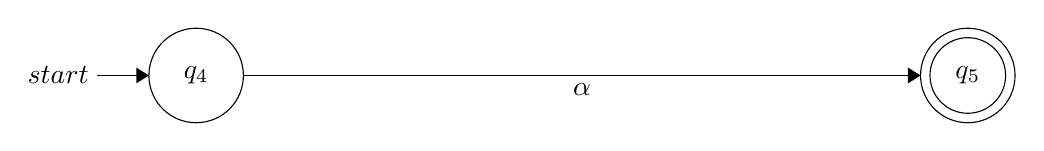
\begin{tikzpicture}[scale=0.2]
\tikzstyle{every node}+=[inner sep=0pt]
\draw [black] (14.3,-27.6) circle (3);
\draw (14.3,-27.6) node {$q_4$};
\draw [black] (63.3,-27.6) circle (3);
\draw (63.3,-27.6) node {$q_5$};
\draw [black] (63.3,-27.6) circle (2.4);
\draw [black] (8,-27.6) -- (11.3,-27.6);
\draw (7.5,-27.6) node [left] {$start$};
\fill [black] (11.3,-27.6) -- (10.5,-27.1) -- (10.5,-28.1);
\draw [black] (17.3,-27.6) -- (60.3,-27.6);
\fill [black] (60.3,-27.6) -- (59.5,-27.1) -- (59.5,-28.1);
\draw (38.8,-28.1) node [below] {$\alpha$};
\end{tikzpicture}
\end{center}



\section*{Answer 5}

The given NFA which N is

\begin{center}
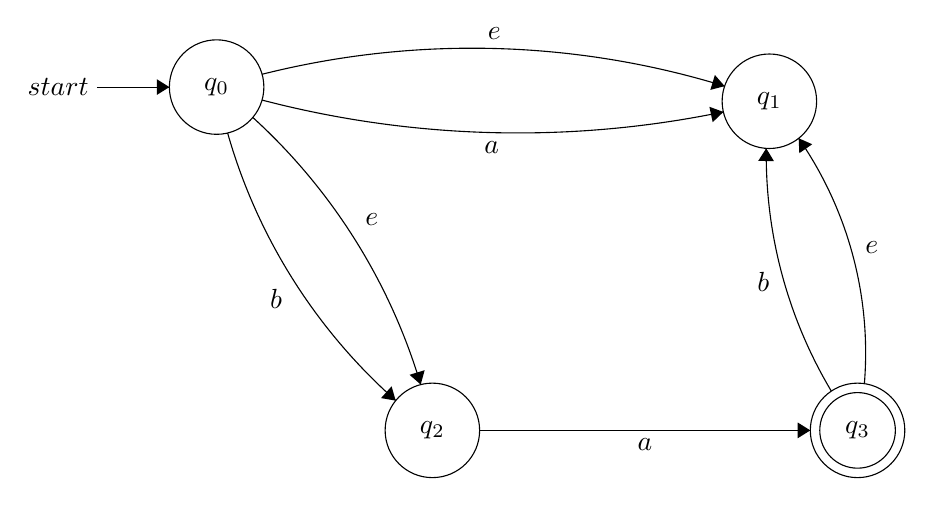
\begin{tikzpicture}[scale=0.2]
\tikzstyle{every node}+=[inner sep=0pt]
\draw [black] (21.6,-12.1) circle (3);
\draw (21.6,-12.1) node {$q_0$};
\draw [black] (56.7,-13) circle (3);
\draw (56.7,-13) node {$q_1$};
\draw [black] (35.3,-33.9) circle (3);
\draw (35.3,-33.9) node {$q_2$};
\draw [black] (62.3,-33.9) circle (3);
\draw (62.3,-33.9) node {$q_3$};
\draw [black] (62.3,-33.9) circle (2.4);
\draw [black] (14,-12.1) -- (18.6,-12.1);
\draw (13.5,-12.1) node [left] {$start$};
\fill [black] (18.6,-12.1) -- (17.8,-11.6) -- (17.8,-12.6);
\draw [black] (24.487,-11.287) arc (104.15757:72.90483:54.537);
\fill [black] (53.86,-12.04) -- (53.24,-11.33) -- (52.95,-12.28);
\draw (39.24,-9.12) node [above] {$e$};
\draw [black] (53.778,-13.677) arc (-78.29372:-104.64388:64.283);
\fill [black] (53.78,-13.68) -- (52.89,-13.35) -- (53.1,-14.33);
\draw (39.07,-15.52) node [below] {$a$};
\draw [black] (23.897,-14.028) arc (47.6875:16.60633:37.394);
\fill [black] (34.56,-30.99) -- (34.81,-30.08) -- (33.85,-30.37);
\draw (31.01,-20.49) node [right] {$e$};
\draw [black] (32.975,-32.006) arc (-131.57265:-164.13353:35.787);
\fill [black] (32.97,-32.01) -- (32.71,-31.1) -- (32.04,-31.85);
\draw (25.79,-25.57) node [left] {$b$};
\draw [black] (60.634,-31.407) arc (-149.18775:-180.81295:29.282);
\fill [black] (56.5,-15.99) -- (55.99,-16.79) -- (56.99,-16.8);
\draw (56.73,-24.5) node [left] {$b$};
\draw [black] (58.558,-15.353) arc (34.70011:-4.70082:23.924);
\fill [black] (58.56,-15.35) -- (58.6,-16.3) -- (59.42,-15.73);
\draw (62.76,-22.27) node [right] {$e$};
\draw [black] (38.3,-33.9) -- (59.3,-33.9);
\fill [black] (59.3,-33.9) -- (58.5,-33.4) -- (58.5,-34.4);
\draw (48.8,-34.4) node [below] {$a$};
\end{tikzpicture}
\end{center}

\subsection*{a.}

If we use the algorithm, we should write the states which are

$E(q_0) = {q_0,q_1,q_2}$ \\
$E(q_1) = {q_1}$ \\
$E(q_2) = {q_2}$ \\
$E(q_3) = {q_1, q_3}$ \\

We can find those by looking the states, adding the states that is reachable with empty transitions.

The state which is ${q_0,q_1,q_2}$ should be initial states since  $q_0$ was the inital state of N.

Then we will look the transtion function.

$\delta({q_0,q_1,q_2},a) = E(q_1) \cup E(q_3) \cup \emptyset= {q_1, q_3}$ \\
$\delta({q_0,q_1,q_2}, b) = E(q_2) \cup \emptyset \cup \emptyset = {q_2}$ \\

$\delta({q_1,q_3},a) = \emptyset \cup \emptyset = \emptyset$ \\
$\delta({q_1, q_3},b) = \emptyset \cup E(q_1) = {q_1}$ \\

$\delta({q_2},a) = E(q_3) = {q_1, q_3}$ \\
$\delta({q_2},b) = \emptyset$ \\

$\delta({q_1}, a) = \emptyset $ \\
$\delta({q_1},b) = \emptyset$ \\

$\delta(\emptyset, a) = \emptyset$ \\
$\delta(\emptyset, b) = \emptyset$ \\

With using new states and new transitions, we get the equivalent DFA which follows

\begin{center}
\begin{tikzpicture}[scale=0.2]
\tikzstyle{every node}+=[inner sep=0pt]
\draw [black] (20.1,-10.4) circle (3);
\draw (20.1,-10.4) node {${q_0,q_1,q_2}$};
\draw [black] (52.7,-10.4) circle (3);
\draw (52.7,-10.4) node {${q_1,q_3}$};
\draw [black] (52.7,-10.4) circle (2.4);
\draw [black] (28.9,-39.5) circle (3);
\draw (28.9,-39.5) node {${q_2}$};
\draw [black] (74.6,-26.9) circle (3);
\draw (74.6,-26.9) node {${q_1}$};
\draw [black] (56.4,-43.2) circle (3);
\draw (56.4,-43.2) node {$\emptyset$};
\draw [black] (12.2,-10.4) -- (17.1,-10.4);
\draw (11.7,-10.4) node [left] {$start$};
\fill [black] (17.1,-10.4) -- (16.3,-9.9) -- (16.3,-10.9);
\draw [black] (23.1,-10.4) -- (49.7,-10.4);
\fill [black] (49.7,-10.4) -- (48.9,-9.9) -- (48.9,-10.9);
\draw (36.4,-10.9) node [below] {$a$};
\draw [black] (30.8,-37.18) -- (50.8,-12.72);
\fill [black] (50.8,-12.72) -- (49.91,-13.02) -- (50.68,-13.66);
\draw (41.36,-26.38) node [right] {$a$};
\draw [black] (31.79,-38.7) -- (71.71,-27.7);
\fill [black] (71.71,-27.7) -- (70.8,-27.43) -- (71.07,-28.39);
\draw (52.54,-33.76) node [below] {$b$};
\draw [black] (55.1,-12.21) -- (72.2,-25.09);
\fill [black] (72.2,-25.09) -- (71.87,-24.21) -- (71.26,-25.01);
\draw (62.65,-19.15) node [below] {$b$};
\draw [black] (53.444,-13.306) arc (13.57683:-0.70476:108.865);
\fill [black] (56.48,-40.2) -- (56.99,-39.41) -- (55.99,-39.4);
\draw (56.46,-26.55) node [right] {$a$};
\draw [black] (73.508,-29.692) arc (-24.91091:-71.39356:24.176);
\fill [black] (59.3,-42.42) -- (60.21,-42.64) -- (59.89,-41.69);
\draw (68.67,-38.01) node [below] {$a$};
\draw [black] (72.37,-28.9) -- (58.63,-41.2);
\fill [black] (58.63,-41.2) -- (59.56,-41.04) -- (58.9,-40.29);
\draw (64.49,-34.56) node [above] {$b$};
\draw [black] (20.97,-13.27) -- (28.03,-36.63);
\fill [black] (28.03,-36.63) -- (28.28,-35.72) -- (27.32,-36.01);
\draw (23.73,-25.56) node [left] {$b$};
\draw [black] (55.59,-46.077) arc (12.01279:-275.98721:2.25);
\draw (50.93,-48.71) node [below] {$a$};
\fill [black] (53.62,-44.31) -- (52.74,-43.98) -- (52.95,-44.96);
\draw [black] (58.912,-44.818) arc (84.94792:-203.05208:2.25);
\draw (60.87,-49.49) node [below] {$b$};
\fill [black] (56.64,-46.18) -- (56.08,-46.93) -- (57.07,-47.02);
\end{tikzpicture}
\end{center}

\subsection*{b.}

If we look the accepted state, which is ${q_1,q_3}$ the language A is only accepted strings which are "a" or "ba". The complement of that language is the set of strings which are not "a" and "ba". The regular expression of the complement of the language which is $\bar{L}$ \\
$= e \cup b \cup (a(a \cup b) \cup bb \cup ba(a \cup b))(a \cup b)^*$ \\
which is also $\bar{L} = \{w \in \sum^* : w\  is\  not\  "a"\  and\  "ba" \}$




\section*{Answer 6}

We can think $L_1 - L_2$ as $L_1 \cap \overline{L_2}$ and also as $\overline{(\overline{L_1} \cup L_2)}$ \\



Assume that the DFA $M_1$ = $\{K_1,\sum_1, \delta_1,s_1,F_1\}$ recognizes language one which is $L_1$ and $M_2$ = $\{K_2,\sum_2, \delta_2,s_2,F_2\}$ recognizes language two which is $L_2$ \\

After getting the complement of the $M_1$ which is DFA that recognizes $L_1$, we get the $\overline{M_1}$. \\
Then add the new initial state which is lets say $s_0$. \\
Then add empty transitions to $\overline{M_1}$'s inital state and $M_2$'s initial state. \\
When we did these operations, we will get $\overline{M_1} \cup M_2$.
After that, we can use the algorithm that can change NFA to DFA. By using this algorithm we can get $M_0 = \overline{M_1} \cup M_2$ \\
After that, if we get the complemt of $M_0$, we get  $M_0$ =$\overline{(\overline{M_1} \cup M_2)}$
which recognizes $\overline{(\overline{L_1} \cup L_2)}$ which is equivalent to $L_1 - L_2$. \\
Since we find $M_0$ which recognizes $L_1 - L_2$, we can easily say that $L_1 - L_2$ is regular language since it is recognized by finite automaton which is $M_0$.



\section*{Answer 7}

\subsection*{a.}

Assume the given language which is $L = \{w \in \{a,b\}^{*} : f(a,w) = n^{2} for some n \in N \}$ \\

The question want us to use pumping lemma. \\

By using pumping lemma we can say that there is an integer $k \geq 1$ such that for any string w, $|w| > k$, and the string can be splitted such as  w = xyz such that the length of xy , $|xy| \leq k$, is less than or equal to k and $xy^iz \in$ L for all i $\geq 0$

Then, take $w = b^{k - n^2}a^2a^{n^2-2}b^l$ where l is a positive number, $l > 0$. It is obvius that w is in the language L because it contains $n^2$ a's. We can the string w as $x = b^{k - n^2}a^2$ y = $a^{n^2-2}$ and $z = b^l$. Then, we can use pumping lemma to claim $xy^iz \in$ L for all i $\geq 0$ because the length of the is greater than k,$|w| = k + l > l$, the length of the string xy is less than or equal to k,$|xy| = k \leq k$, and we assumed that the L is regular language.
But, if we take i = 0, we will get xz = $b^{k - n^2}a^2b^l$. By pumping lemma that string must be in the language, however, that is not possible since the string only contains 2 a's, since 2 is not a square of a natural number. The fact that L is not a regular language is proved by the contradiction and pumping lemma. 






\end{document}

​

